\chapter[Mutation]{Mutation testing}
\label{cap:preliminares.mutation}

\emph{Mutation testing} es un criterio de cobertura que puede ser considerado de \emph{caja blanca}, en donde las metas a cubrir por la test suite, est\'an representadas por fallas artificiales, que deben ser detectadas por la test suite bajo evaluaci\'on. Las fallas artificiales se representan por variantes del programa original, en donde cada una tiene un cambio sint\'actico simple, representando un defecto. Cada variante se denomina \emph{mutante}, mientras que la falla artificial asociada, se llama \emph{mutaci\'on}. Cuantos, de los mutantes generados, son detectados por la test suite, es el valor asociado a este criterio, y se denomina \emph{mutation score}.

Las fallas artificiales involucradas en mutation testing son producidas basadas en \emph{operadores de mutaci\'on}. Un operador de mutaci\'on define los cambios sint\'acticos que se van a producir a partir de un programa, t\'ipicamente eligiendo tipos particulares de expresiones en el mismo, y llevando a familias de mutantes. Dos ejemplos tradicionales de operadores de mutaci\'on son \emph{reemplazo de operadores relacionales}, el cual reemplaza un operador relacional por todos los otros soportados por el lenguaje de programaci\'on utilizado, y \emph{reemplazo de operadores aritm\'eticos}, que realiza cambios similares pero sobre operadores aritm\'eticos. Las mutaciones $1\Delta$, $2\Delta$ and $3\Delta$ en la Figura \ref{figures.examples.mutations} corresponden a reemplazo de operadores relacionales, mientras que $4\Delta$ corresponde a reemplazo de operadores aritm\'eticos.

\begin{figure}[t]
	\begin{lstlisting}[frame=tlrb, mathescape=true]
  int countEven( int[] input ) {
    int count = 0;
    for (int i = 0; i < input.length; i++) {
    $1\Delta$for (int i = 0; i <= input.length; i++) {
    $2\Delta$for (int i = 0; i != input.length; i++) {
      int value = input[i];
      if (value % 2 == 0) {
      $3\Delta$ if (value % 2 != 0) {
        count = count + 1;
        $4\Delta$ count = count / 1;
      }
    }
    return count;
  }
	\end{lstlisting}
	\caption{Ejemplos de un programa y posibles mutaciones}
	\label{figures.examples.mutations}
\end{figure}

Como con cualquier criterio, mientras mas cercano al 100\% sea el valor asociado, m\'as confianza se puede tener en la calidad de la test suite evaluada. En el caso de mutation testing, este valor aumenta mientras m\'as mutantes sean detectados y disminuye en caso contrario, sin embargo existen situaciones que afectan de manera negativa a la confianza sobre este valor. Ciertas fallas son triviales de detectar, ya sea por que causan que la compilaci\'on o la ejecuci\'on (bajo cualquier entrada) falle, o solo requieren alcanzabilidad para hacerlo, por ejemplo \lstinline|if (c) x = array[-1];|, solo requiere una entrada que satisfaga \emph{c} para detectar la falla, ni siquiera es necesario un or\'aculo para evaluar el resultado. Las fallas triviales aumentan el mutation score sin implicar una mejora en la calidad de la test suite. En el espectro opuesto, pueden haber fallas artificiales que tengan el mismo comportamiento sem\'antico que el c\'odigo original, por ejemplo \lstinline|for (int i = 0; i < 10; i++)| es equivalente a \lstinline|for (int i = 0; i < 10; ++i)|. Estos mutantes son llamados equivalentes y por lo tanto indistinguibles del programa original, lo que genera metas que no pueden ser cubiertas, que a su vez disminuye el valor de mutation score, pero la test suite no tiene una peor calidad por no ser capaz de detectar estos mutantes. Finalmente un valor alto de mutation score no significa nada si no existe una relaci\'on entre detectar fallas artificiales y reales.

\section{Operadores de mutaci\'on suficientes}
\label{sec:preliminares.mutation.sufficient}

El estudio llevado a cabo en \cite{bibliography.mutation.selection.Offutt96}, evalu\'o el conjunto de operadores de mutaci\'on utilizados por \emph{Mothra}, una herramienta de mutation testing para el lenguaje Fortran-77. Llegando al siguiente conjunto de operadores considerados como suficientes:

\begin{description}[leftmargin=8em,style=nextline]
	\item[ABS] Modifica cada expresi\'on aritm\'etica por 0, un valor positivo, y un valor negativo.
	\item[AOR] Reemplaza cada operador aritm\'etico con todos los operadores legales.
	\item[LCR] Reemplaza operadores l\'ogicos o condicionales por otros v\'alidos.
	\item[ROR] Reemplaza operadores relacionales.
	\item[UOI] Inserta operadores unarios en expresiones compatibles.
\end{description}

Si bien otros estudios sobre conjunto suficiente de operadores, entre ellos \cite{bibliography.mutation.selection.ASN2008}, se han realizado. Particularmente \'este concluye en un conjunto muy similar al anterior, con la diferencia que la herramienta de mutaci\'on ofrece una mayor cantidad de operadores de mutaci\'on, que en muchos casos est\'an inclu\'idos en los anteriores.

Cabe destacar que estos estudios siempre cuentan con la misma amenaza de validez, el hecho de realizar el estudio bajo un conjunto de programas determinados con un conjunto de tests particulares. Sin embargo, todos llegan al mismo conjunto de cambios, ya sean realizados por los mismos operadores o por operadores similares.

\section{Propiedades de operadores de mutaci\'on}
\label{sec:preliminares.mutation.opevaluation}

En principio, un operador de mutaci\'on es una funci\'on que aplica a elementos particulares de un programa, ya sea c\'odigo fuente o binarios, y genera versiones modificadas de \'estos. Un operador a su vez deber\'ia tener un objetivo claro, como emular cierto tipo de fallas. Sin embargo para que mutation testing sea un criterio efectivo, algunas propiedades deben ser tenidas en cuenta. \textbf{Tiempo, y otros recursos}, obligan a que el conjunto de mutantes generados se mantenga acotado, de la misma forma en que es necesario acotar el conjunto de tests a utilizar para evaluar un programa. \textbf{Efectividad}, un criterio de cobertura para tests es utilizado para evaluar la calidad de los mismos, precisamente con respecto a cuan efectivos son para detectar potenciales fallas en el programa bajo prueba. Mutation testing tiene un problema similar, dado que la cantidad de fallas artificiales (mutaciones) con las que se va a evaluar a un test suite es finita, genera a su vez, una necesidad de evaluar a \'estas con respecto a su efectividad para evaluar a una test suite para el programa bajo prueba, espec\'ificamente, c\'omo el conjunto de mutantes obliga a la test suite a ejercitar al programa. \textbf{Representaci\'on de fallas reales}, parece extra\~no que un conjunto de mutantes sea muy efectivo para evaluar un conjunto de tests, pero que no represente fallas reales. Sin embargo, efectividad en la ejercitaci\'on de un test suite solo permite evaluar cuan capaz es \'este de detectar cambios sem\'anticos. Mientras que, una alta efectividad para esto, en el contexto de mutantes, no implica que se mantenga para fallas reales, principalmente por que mutation testing intenta emular fallas complejas mediante fallas simples. Un problema ortogonal a estas propiedades, es la confianza, o cuan significativo es el valor de mutation score que resulta de un conjunto particular de mutantes. A continuaci\'on vamos a mencionar que caracter\'isticas afectan o est\'an relacionadas con las propiedades anteriores, y como es posible medirlas.

\subsection{Equivalencia}

Equivalencia [entre dos programas] es una propiedad definida bajo la relaci\'on \texttt{Eq(P, P$\prime$) : $\nexists$ E : P(E) != P$\prime$(E)}, la cual establece que dos programas \texttt{P} y \texttt{P$\prime$} son equivalente si no existe un escenario \texttt{E} tal que el comportamiento de ambos programas sea distinto. \'Esta es una relaci\'on indecidible, por lo que m\'etodos incompletos son utilizados. Dentro de mutation testing, equivalencia puede encontrarse entre un mutante y el programa original, un caso indeseable ya que \'estos disminuyen el valor del mutation score sin significar una deficiencia de parte de la test suite en detectar ciertas fallas artificiales. Otro caso de equivalencia se da entre mutantes, un caso en donde ambos mutantes son detectados por la test suite, sin embargo al ser equivalente incrementan el valor del mutation score sin significar una mejora de parte de la test suite en detectar m\'as fallas artificiales.

Dentro de la investigaci\'on sobre la detecci\'on (evaluaci\'on) de esta caracter\'istica y su impacto en el an\'alisis de test suites usando mutation testing, \cite{biblography.mutation.evaluation.equivalent.Schuler+10} propone la utilizaci\'on de diferencia en cobertura de c\'odigo y an\'alisis de flujo de datos para determinar potencial equivalencia. Mientras que  \cite{biblography.mutation.evaluation.equivalent.Just+13} utiliza detecci\'on de restricciones condicionales para alcanzar el c\'odigo mutado y \emph{SAT Solving} para determinar si es posible satisfacer dichas restricciones al tiempo que se obtiene un valor distinto al del programa original en ese punto, lo que es similar en principio a \emph{weak mutation}, en donde se considera que un mutante es detectado si en el estado siguiente a la mutaci\'on se detecta una diferencia con el del programa original, pero a\~nadiendo control de alcanzabilidad y una verificaci\'on exhaustiva acotada para detectar si es posible que exista una diferencia.
En \cite{biblography.mutation.evaluation.equivalent.Grun+09} observan que manualmente, para los casos de estudios utilizados, un programador avanzado tarda aproximadamente 15 minutos en promedio para analizar mutantes equivalentes. Y claramente la existencia de equivalentes disminuye artificialmente el mutation score dando la falsa impresi\'on de que es necesario agregar m\'as tests. Si analizamos el impacto de equivalencia entre mutantes, podemos diferenciar dos casos particulares: equivalencia entre mutantes detectados, \emph{m$_1$} y \emph{m$_2$} son ambos detectados por la test suite bajo evaluaci\'on, sin embargo son equivalentes entre s\'i, esta situaci\'on lleva a un incremento del mutation score por b\'asicamente detectar m\'as de una vez el mismo mutante; equivalencia entre mutantes no detectados, \emph{m$_1$} y \emph{m$_2$} son ambos mutantes sobrevivientes, esto lleva a un decremento del mutation score por b\'asicamente fallar en detectar el mismo mutante dos veces.

\subsection{Dificultad de detecci\'on}

As\'i como los mutantes equivalentes son indeseables por ser imposibles de detectar, los mutantes que son solo detectables por un conjunto peque\~no de tests, son altamente deseables. \'Estos son denominados \emph{stubborn} \cite{bibliography.mutation.evaluation.stubbornHieronsHD99}. La detecci\'on de estos mutantes requiere tests de ``mejor calidad'', y si bien existen estudios que eval\'uan la generaci\'on de stubborns por operador \cite{bibliography.mutation.evaluation.stubborn}, esto depende del conjunto de programas utilizados y los tests asociados. Con respecto a este obst\'aculo, en \cite{bibliography.mutation.evaluation.hardnessVisser}, proponen el uso de \emph{model counting} sobre programas m\'as simples pero utilizando un estudio m\'as exhaustivo. Algunas medidas preventivas para evitar generar mutantes triviales de detectar incluyen controles m\'as estrictos en la generaci\'on, para evitar mutantes que no compilen, por ejemplo, AOIS, un operador que inserta \lstinline|++| y \lstinline|--| en variables aritm\'eticas, puede generar mutantes inv\'alidos si no comprueba que la variable a mutar no es una constante. La raz\'on por la cual detectar o prevenir una baja dificultad de detecci\'on para un conjunto de mutantes, es que es dif\'icil definir precisamente a esta dificultad. Mientras que equivalencia es una propiedad binaria, en el sentido de que, dos programas son o no equivalentes, la dificultad de detecci\'on es una propiedad muy dif\'icil de definir. 

\subsection{Subsuma}

\emph{Subsumption}, la relaci\'on entre mutantes con respecto a los tests que los detectan, da lugar a mutantes redundantes. Esto es, los tests que detectan al mutante subsumido, incluyen a todos aquellos que detectan al que subsume, es decir, el mutante subsumido eval\'ua de manera menos espec\'ifica a los tests, ya que es detectado por una mayor cantidad, mientras que el que subsume eval\'ua tests m\'as espec\'ificos. Esto lleva a mutantes redundantes y representa una forma indirecta de evaluar la dificultad de detecci\'on, los mutantes que subsumen a otros pero no son a su vez subsumidos, son detectados por pocos tests. Presentado inicialmente en \cite{bibliography.mutation.selection.Offutt96}, mutant subsumption es utilizado por \cite{bibliography.mutation.minimizing.dynamicsubsumption} y \cite{bibliography.mutation.evaluation.JustKA17} para evaluar utilidad de mutantes dentro de mutation analysis. Partiendo de que los mutantes utilizados en mutation testing, tienen como objetivo ejercitar a un conjunto de tests para evaluar de manera indirecta la capacidad de los mismos en detectar potenciales fallas reales, aquellos que ejerciten de manera m\'as espec\'ifica a los tests, son considerados entonces, mejores. Un ejemplo de subsuma de mutantes se puede ver en las figuras \ref{figures.examples.subsumptionTable} y \ref{figures.examples.subsumptionGraph}.

\begin{figure}
	\begin{displaymath}
		\begin{array}{llll}
			Tests & M1 & M2 & M3  \\
			1     & \bullet  & \bullet  &     \\
			2     &    & \bullet  & \bullet   \\
			3     &    &    & \bullet  
		\end{array}
	\end{displaymath}
	\caption{Ejemplo de subsuma de mutantes}
	\label{figures.examples.subsumptionTable}
\end{figure}

\begin{figure}
	\begin{center}
		\usetikzlibrary{positioning}
		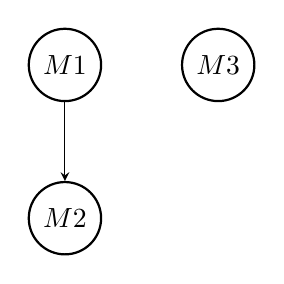
\begin{tikzpicture}[xscale=10, yscale=10,>=stealth]
		\tikzstyle{v}=[circle, minimum size=1mm,draw,thick]
		\node[v] (M1) {$M1$};
		\node[v] (M2) [below=of M1] {$M2$};
		\node[v] (M3) [right=of M1] {$M3$};
		\draw [->] (M1) to (M2);
		\end{tikzpicture}
	\end{center}
	\caption{Grafo de subsuma basado en la Tabla \ref{figures.examples.subsumptionTable}}
	\label{figures.examples.subsumptionGraph}
\end{figure}

\subsection{Acoplamiento}

\emph{Coupling}, el acoplamiento entre fallas reales y mutantes es una propiedad altamente deseable, sin la misma, mutation testing perder\'ia su utilidad al desaparecer la correlaci\'on entre un mutation score alto y una buena capacidad de parte de la test suite para detectar fallas reales. El trabajo m\'as importante sobre este tema, y uno que nos representa una motivaci\'on importante para el desarrollo de nuestro operador de mutaci\'on presentado en esta tesis, es \cite{bibliography.mutation.evaluation.valid-substitute}. El acoplamiento entre mutantes y fallas reales es una relaci\'on que especifica que si un conjunto de tests detecta un conjunto de mutantes, entonces va a detectar una falla real. Por el otro lado, el acoplamiento entre mutantes, representa una situaci\'on indeseable, al ser similar al caso de equivalencia entre mutantes. Una manera si bien poco exigente, para medir acoplamiento entre un programa y un conjunto de mutantes, es evaluar si los tests que detectan las fallas, son los mismos que detectan al conjunto de mutantes. En el trabajo previo, uno de las exigencias adicionales fue solo mutar el c\'odigo asociado a la reparaci\'on de la falla real.

%\section{High order}
%
%\texttt{High Order}, la combinaci\'on de mutaciones, generada al aplicar operadores de mutaci\'on m\'as de una vez al generar un mutante, se denominan mutaciones de alto order mientras que aquellas que la forman, se las llama de primer orden. Si bien en principio esto agregar\'ia una gran cantidad de nuevos mutantes\footnote{Usualmente la cantidad de mutantes al aplicar m\'as de una mutaci\'on por mutante est\'a acotada por M$_0^G$ en donde \texttt{M$_0$} son la cantidad de mutantes de primer orden y \texttt{G} son la cantidad de mutaciones por mutante}, los estudios actuales que se enfocan en esta t\'ecnica concluyen que estos mutantes de alto orden representan fallas artificiales m\'as sutiles y que subsumen a una gran cantidad de mutantes de primer orden. [AGREGAR]

\section{Dynamic Mutant Subsumption como m\'etrica}
\label{sec:preliminares.mutation.whysubsumption}

En la secci\'on anterior presentamos las propiedades deseables en los mutantes generados por un operador de mutaci\'on, y algunas formas de evaluar el grado en que \'estas se cumplen. Sin embargo, al evaluar operadores de mutaci\'on con respecto a otros, o t\'ecnicas de selecci\'on de mutantes, la utilizaci\'on de m\'etricas como diferencia entre mutation score, cantidad de mutantes equivalentes generados (o evitados), ``dureza'' de mutantes (cuantos tests logra sobrevivir el mutante antes de ser detectado) y cantidad de mutantes, son las m\'as utilizadas.

En esta tesis se plantea utilizar \emph{Dynamic Mutant Subsumption} como una de las m\'etricas principales para evaluar a \emph{prvo} con respecto al conjunto de operadores suficientes implementados en \emph{$\mu$Java}. La raz\'on de esto se debe a la cantidad de informaci\'on que permanece oculta al utilizar m\'etricas usuales.

Para utilizar un caso particular sobre el cual discutir las desventajas de las m\'etricas usuales vamos a referirnos a un trabajo publicado sobre un operador de mutaci\'on para fortalecer y debilitar expresiones booleanas \cite{bibliography.mutation.operators.beeBridaS17}. \'Este surge de la intuici\'on de que los operadores que afectan expresiones booleanas al modificar operadores (\emph{ROR}, \emph{COR}, \emph{COI}, entre otros) o reemplazar partes de la expresi\'on, como el caso de \emph{ROR} que reemplaza una expresi\'on boolena por las constantes \emph{True} y \emph{False}, generan cambios ``muy gruesos'' como cambiar una condici\'on de \textbf{a > b} por \textbf{a < b}, mientras que una modificaci\'on del estilo \textbf{a > b \&\& c} nos parece que puede llevar a mutantes m\'as sutiles. En este estudio utilizamos el mismos conjunto de operadores contra los que comparamos \emph{prvo}, y evaluamos como la utilizaci\'on de \emph{BEE} afectaba a las siguientes m\'etricas:
\begin{description}[leftmargin=8em,style=nextline]
	\item[Mutation score] El decremento en el valor obtenido de mutation score al utilizar a \emph{BEE} servir\'ia como indicador de que mutantes m\'as dif\'iciles fueron generados. Mientras que un incremento indicar\'ia el aumento de mutantes m\'as triviales de detectar.
	\item[Cantidad de mutantes] Dado que en el peor caso es necesario ejecutar todos los tests para cada mutante (suponiendo un an\'alisis solo centrado en mutation score) los recursos utilizados por mutation testing, entre ellos tiempo, est\'an directamente relacionados a la cantidad de mutantes generados, todo operador deber\'ia ser evaluado con respecto al costo asociado, es decir, cuantos mutantes agrega al an\'alisis.
	\item[Dureza (toughness)] La cantidad de tests que un mutante es capaz de ``sobrevivir'', no ser detectado por, puede servir como una m\'etrica para evaluar cuan dif\'icil de detectar resulta. Analizar como cambia la dureza promedio de los mutantes detectados al agregar un operador (en este caso \emph{BEE}) permite evaluar la dificultad de detecci\'on de los mutantes agregados por el mismo.
	\item[Mutantes equivalentes] Una caracter\'istica negativa de un operador es cuantos mutantes equivalentes produce, \'estos son mutantes que si bien son distintos sint\'acticamente, son sem\'anticamente equivalentes al programa original, y por lo tanto imposibles de detectar.
	\item[Mutantes dif\'iciles de matar (stubborn)] La generaci\'on de mutantes dif\'iciles de matar (stubborn) es una caracter\'istica altamente deseable para un operador de mutaci\'on. Sin embargo representa una propiedad muy compleja para analizar, principalmente por la dificultad en dar una definici\'on apropiada, una de \'estas corresponde a la propuesta por Xiangjuan Yao et al. \cite{bibliography.mutation.evaluation.stubborn}: un mutante dif\'icil de matar es aquel para el cual existe un tests que es capaz de detectarlo pero no est\'a presente en un test suite ``suficientemente bueno'' el cual luego define como un test suite con 100\% de cobertura de ramas. Aunque finalmente se utilizan definiciones m\'as relajadas como la utilizaci\'on de testing exhaustivo acotado (considerar todas las entradas dentro de ciertas cotas) o generaci\'on de test suites mediante herramientas como \emph{EvoSuite} con una cobertura de ramas por encima del 80\%.
\end{description}

La evaluaci\'on presentada en \cite{bibliography.mutation.operators.beeBridaS17} utiliza estas m\'etricas para la evaluaci\'on del nuevo operador, y si bien los resultados no fueron negativos, \'estos no parecen mostrar una clara ventaja de utilizar el operador, aunque la motivaci\'on detr\'as del mismo as\'i como su definici\'on, parecer\'ia indiciar que el mismo tiene potencial. Un problema que tienen estos resultados es la cantidad de informaci\'on que permanece oculta. Como mencionamos en la secci\'on \ref{sec:preliminares.mutation.opevaluation}, el valor de mutation score se ve altamente afectado por: mutantes equivalentes, que disminuyen el valor sin significar una baja calidad de parte de los tests; mutantes triviales, que aumentan el valor mediante mutaciones que son triviales de detectar y no resultan en una evaluaci\'on apropiada de los tests; acoplamiento entre mutantes, cuando la detecci\'on de una mutaci\'on implica la detecci\'on de otra o cuando dos mutantes son equivalentes entre s\'i incrementan el mutation score por (en cierto modo) mutantes repetidos y lo mismo puede causar un decremento repetido en este valor.

El an\'alisis de mutantes equivalentes es un problema indecidible, an\'alisis manuales siguen siendo uno de los enfoques m\'as utilizados aunque sigue siendo una propiedad com\'unmente evaluada y con una gran importancia en comparaci\'on de operadores de mutaci\'on o t\'ecnicas de selecci\'on de mutantes.

La dificultad de un mutante por el otro lado, es una propiedad que si bien ser\'ia interesante evaluar, resulta muy dif\'icil de definir, Visser presenta en \cite{bibliography.mutation.evaluation.hardnessVisser} un estudio sobre la dificultad de detectar mutantes el cual utiliza \emph{model counting} para evaluar la cantidad de escenarios (de manera exhaustiva, en un conjunto acotado) que logran diferenciar a un mutante del programa original. Este enfoque no resulta pr\'actico, algo que es mencionado en el trabajo anterior, y solo es posible en programas muy simples.

El uso de \emph{Dynamic Mutant Subsumption} a sido utilizado previamente para minimizar conjuntos de mutantes en \cite{bibliography.mutation.minimizing.dynamicsubsumption} y para medir la efectividad de un conjunto de mutantes en \cite{bibliography.mutation.efectiveness.dynamicsubsumption}, este \'ultimo trabajo sugiere la utilizaci\'on de dynamic mutant subsumption como forma de comparar operadores de mutaci\'on y/o t\'ecnicas de selecci\'on de mutantes. Una ventaja inicial de utilizar esta t\'ecnica es que la definici\'on es clara, un mutante subsume a otro si ambos son detectados y los tests que detectan al primero tambi\'en detectan al segundo. A su vez, la conclusi\'on de que los mutantes subsumidos son redundantes se relaciona a la existencia de otro/s mutantes que ejercitan al conjunto de tests de manera m\'as espec\'ifica (son detectados por menos tests), y los mutantes equivalentes con respecto a subsuma ejercitan varias veces al mismo conjunto de tests, pudiendo elegir un solo representante de \'estos. La dificultad de detecci\'on puede asociarse a subsuma argumentando que si un mutante subsume a otros, es detectado por menos tests, dando la intuici\'on de que requiere tests m\'as espec\'ificos que los mutantes que subsume.

Retomando el estudio sobre el operador \emph{BEE}, cuando realizamos un an\'alisis de subsuma logramos obtener resultados mas significativos con respecto a la utilidad del operador para mutation testing. Las preguntas de investigaci\'on de este trabajo son:
\begin{quote}
	{\it Nuestro operador (BEE) genera mayor cantidad de mutantes dif\'iciles de matar (stubborn) que los operados existentes que debilitan o fortalecen expresiones booleanas?}
\end{quote}
\begin{quote}
	{\it Como nuestro operador (BEE) afecta al an\'alisis de mutaci\'on?}
\end{quote}

Siendo los resultados obtenidos los de las Tablas \ref{tables.examples.bee.paperResults.arraypartition}, \ref{tables.examples.bee.paperResults.binaryheap}, \ref{tables.examples.bee.paperResults.ordset}, \ref{tables.examples.bee.paperResults.treemap}, y \ref{tables.examples.bee.paperResults.trityp}. Estos resultados dieron lugar a la conclusi\'on de que la respuesta a la primer pregunta de investigaci\'on es negativa (\emph{BEE} no parece generar una cantidad importante de mutantes dif\'iciles de matar), mientras que la segunda pregunta se responde de una manera m\'as positiva al indicar que la dificultad de matar los mutantes generados por \emph{BEE} parece mantenerse con respecto al resto de los mutantes (el valor de \emph{toughness} pr\'acticamente no cambia) y que la cantidad de mutantes equivalentes generados se deben a particularidades de algunos casos. Un problema con los resultados utilizados es que parecen estar ocultando informaci\'on. Por esto, al realizar un an\'alisis de los mismos casos utilizados en el trabajo publicado, pero utilizando Dynamic Mutant Subsumption, obtenemos los resultados en la Figura \ref{subsumption-results-bee} que permiten observar que en tres de los cinco casos de estudio (\emph{BinaryHeap}, \emph{OrdSet}, y \emph{TreeMap}) los mutantes generados por \emph{BEE} son dominadores, es decir, corresponden a mutantes no redundantes para evaluar a los tests. En los casos de \emph{BinaryHeap} y \emph{OrdSet} se observa que al menos el 50\% de los mutantes dominadores generador por \emph{BEE} no son equivalentes a otros mutantes dominadores, lo que permite concluir que representan fallas nuevas no generadas por los otros operadores.

Esta comparaci\'on sirve de argumento para utilizar Dynamic Mutant Subsumption como una de las principales t\'ecnicas para evaluar un operador de mutaci\'on.

\begin{table}[]
	\centering
	\scriptsize
	\def\arraystretch{0.95}
	\setlength\tabcolsep{0.5mm}
	\begin{tabular}{c|ccccc|}
		\cline{2-6}
		& Mutantes & Sobrevivientes & Toughness (killed) & Mutation score & Stubborn \\ \hline
		\multicolumn{1}{|c|}{SIN BEE} & 196 & 14 & 0.50 & 92.85\% & 6 \\ \hline
		\multicolumn{1}{|c|}{CON BEE} & 336 & 36 & 0.53 & 89.28\% & 8 \\ \hline
	\end{tabular}
	\caption{Datos de evaluaci\'on de \emph{BEE} para \emph{ArrayPartition} de acuerdo al trabajo presentado en \cite{bibliography.mutation.operators.beeBridaS17}}
	\label{tables.examples.bee.paperResults.arraypartition}
\end{table}

\begin{table}[]
	\centering
	\scriptsize
	\def\arraystretch{0.95}
	\setlength\tabcolsep{0.5mm}
	\begin{tabular}{c|ccccc|}
		\cline{2-6}
		& Mutantes & Sobrevivientes & Toughness (killed) & Mutation score & Stubborn \\ \hline
		\multicolumn{1}{|c|}{SIN BEE} & 454 & 111 & 0.73 & 75.55\% & 65 \\ \hline
		\multicolumn{1}{|c|}{CON BEE} & 889 & 341 & 0.72 & 61.64\% & 163 \\ \hline
	\end{tabular}
	\caption{Datos de evaluaci\'on de \emph{BEE} para \emph{BinaryHeap} de acuerdo al trabajo presentado en \cite{bibliography.mutation.operators.beeBridaS17}}
	\label{tables.examples.bee.paperResults.binaryheap}
\end{table}

\begin{table}[]
	\centering
	\scriptsize
	\def\arraystretch{0.95}
	\setlength\tabcolsep{0.5mm}
	\begin{tabular}{c|ccccc|}
		\cline{2-6}
		& Mutantes & Sobrevivientes & Toughness (killed) & Mutation score & Stubborn \\ \hline
		\multicolumn{1}{|c|}{SIN BEE} & 1278 & 179 & 0.83 & 85.99\% & 160 \\ \hline
		\multicolumn{1}{|c|}{CON BEE} & 2248 & 620 & 0.83 & 72.41\% & 403 \\ \hline
	\end{tabular}
	\caption{Datos de evaluaci\'on de \emph{BEE} para \emph{OrdSet} de acuerdo al trabajo presentado en \cite{bibliography.mutation.operators.beeBridaS17}}
	\label{tables.examples.bee.paperResults.ordset}
\end{table}

\begin{table}[]
	\centering
	\scriptsize
	\def\arraystretch{0.95}
	\setlength\tabcolsep{0.5mm}
	\begin{tabular}{c|ccccc|}
		\cline{2-6}
		& Mutantes & Sobrevivientes & Toughness (killed) & Mutation score & Stubborn \\ \hline
		\multicolumn{1}{|c|}{SIN BEE} & 576 & 160 & 0.93 & 72.22\% & 114 \\ \hline
		\multicolumn{1}{|c|}{CON BEE} & 2536 & 1376 & 0.94 & 45.74\% & 631 \\ \hline
	\end{tabular}
	\caption{Datos de evaluaci\'on de \emph{BEE} para \emph{TreeMap} de acuerdo al trabajo presentado en \cite{bibliography.mutation.operators.beeBridaS17}}
	\label{tables.examples.bee.paperResults.treemap}
\end{table}

\begin{table}[]
	\centering
	\scriptsize
	\def\arraystretch{0.95}
	\setlength\tabcolsep{0.5mm}
	\begin{tabular}{c|ccccc|}
		\cline{2-6}
		& Mutantes & Sobrevivientes & Toughness (killed) & Mutation score & Stubborn \\ \hline
		\multicolumn{1}{|c|}{SIN BEE} & 435 & 109 & 0.98 & 74.94\% & 56 \\ \hline
		\multicolumn{1}{|c|}{CON BEE} & 55 & 115 & 0.98 & 79.27\% & 62 \\ \hline
	\end{tabular}
	\caption{Datos de evaluaci\'on de \emph{BEE} para \emph{TriTyp} de acuerdo al trabajo presentado en \cite{bibliography.mutation.operators.beeBridaS17}}
	\label{tables.examples.bee.paperResults.trityp}
\end{table}

\begin{figure}[t]
	\begin{center}
		\includegraphics[width=12cm]{figures/BEETables.png}
	\end{center}
	\caption{Dynamic subsumption analysis para el operador \emph{BEE}}
	\label{subsumption-results-bee}
\end{figure}